\documentclass[journal,onecolumn]{IEEEtran}
\usepackage{graphicx}
\usepackage{booktabs}
\usepackage{multirow}
\usepackage{float}
\usepackage{placeins}
\usepackage{amsmath}
\usepackage{amssymb}

\graphicspath{{./images/}}

\begin{document}

\title{Supplementary Materials for\\
ADMET-Bench: Task-Dependent Performance of GNNs and Pretrained Models in ADMET Prediction}

\author{}

\maketitle

\renewcommand{\thetable}{S\arabic{table}}
\renewcommand{\thefigure}{S\arabic{figure}}

\section{Architecture-Selection Experiments}
\label{sec:supp_architecture}

This supplementary document reports the preliminary architecture-selection screen used to choose the graph neural network backbone for the main study. Eight message-passing variants (GraphConv, GCN, GAT, GraphSAGE, GIN, TAG, SGC, and TransformerConv) were evaluated on all six benchmark endpoints under the \emph{same} scaffold-split pipeline, target transformations, and evaluation metrics used in the main manuscript. For each architecture and endpoint the reported result is the best of five configurations selected on the validation split (searching over hidden dimension, number of layers, and learning rate), giving $8 \times 6 \times 5 = 240$ training runs in total. Because the screen shares the main study's protocol, the values below are directly comparable to the main-text results; they are provided for transparency and reproducibility and, as discussed in the main text, show that no single architecture dominates across endpoints.

\begin{table}[H]
\centering
\caption{Preliminary classification architecture screen: \emph{validation}-split AUC-ROC and F1 (the model-selection basis), each architecture at its best of five validation-selected configurations (search over hidden dimension, number of layers, and learning rate). Best validation AUC per task in \textbf{bold}. Test-set performance was not used for architecture selection.}
\label{tab:arch_classification}
\small
\setlength{\tabcolsep}{4pt}
\begin{tabular}{lcccc}
\toprule
\textbf{Architecture} & \multicolumn{2}{c}{\textbf{Tox21 (NR-AR)}} & \multicolumn{2}{c}{\textbf{hERG}} \\
 & \textbf{Val AUC} & \textbf{Val F1} & \textbf{Val AUC} & \textbf{Val F1} \\
\midrule
GraphConv & 0.819 & 0.480 & 0.918 & 0.903 \\
GCN & 0.821 & 0.435 & 0.912 & 0.915 \\
GAT & 0.819 & 0.500 & 0.907 & 0.871 \\
GraphSAGE & \textbf{0.854} & 0.421 & 0.903 & 0.918 \\
GIN & 0.844 & 0.500 & 0.884 & 0.933 \\
TAG & 0.821 & 0.444 & 0.892 & 0.897 \\
SGC & 0.829 & 0.500 & \textbf{0.920} & 0.875 \\
Transformer & 0.778 & 0.480 & 0.905 & 0.881 \\
\bottomrule
\end{tabular}
\end{table}

\begin{table}[H]
\centering
\caption{Regression architecture screen: average rank across the four ADME regression datasets by \emph{validation} R$^2$ (lower rank is better), the basis on which the backbone was selected; each architecture at its best of five validation-selected configurations (search over hidden dimension, number of layers, and learning rate). Per-dataset validation R$^2$ shown; the final column gives mean \emph{test} R$^2$ as a post-hoc reference only (not used for selection). GraphConv (deployed backbone) in \textbf{bold}.}
\label{tab:arch_regression}
\small
\setlength{\tabcolsep}{4pt}
\begin{tabular}{lcccccccc}
\toprule
\textbf{Arch.} & \textbf{Avg Rank} & \textbf{Caco-2} & \textbf{Half-Life} & \textbf{Clear. Hep.} & \textbf{Clear. Mic.} & \textbf{Test R$^2$} & \textbf{Params} & \textbf{Time (s)} \\
\midrule
GraphSAGE & 3.00 & 0.597 & 0.434 & 0.316 & 0.175 & 0.096 & 662k & 7.3 \\
Transformer & 3.25 & 0.606 & 0.335 & 0.327 & 0.208 & $-$0.197 & 316k & 16.4 \\
TAG & 4.25 & 0.582 & 0.407 & 0.228 & 0.279 & 0.226 & 1059k & 12.2 \\
\textbf{GraphConv} & 4.25 & 0.575 & 0.460 & 0.267 & 0.081 & $-$0.673 & 81k & 7.1 \\
GCN & 4.75 & 0.534 & 0.447 & 0.247 & 0.137 & $-$0.673 & 399k & 12.8 \\
GAT & 5.00 & 0.513 & 0.483 & 0.233 & 0.122 & 0.128 & 1067k & 14.9 \\
SGC & 5.50 & 0.560 & 0.426 & 0.194 & 0.159 & 0.006 & 463k & 12.6 \\
GIN & 6.00 & 0.625 & 0.368 & 0.157 & 0.058 & $-$1.572 & 113k & 6.2 \\
\bottomrule
\end{tabular}
\end{table}

Ranked by \emph{validation} performance (the only leak-free selection signal), no architecture dominates: the eight backbones span a narrow average regression rank ($3.0$--$6.0$; Table~\ref{tab:arch_regression}) and cluster tightly on the classification endpoints (validation AUC $0.78$--$0.85$ on Tox21 and $0.90$--$0.92$ on hERG; Table~\ref{tab:arch_classification}). Like every backbone, GraphConv is unstable on the weakly-learnable clearance and half-life endpoints, an instability that is a property of the endpoints rather than of any single backbone. The validation ranking is moreover a poor predictor of test performance: the best validation-ranked regression backbone (GraphSAGE) reaches only mean test R$^2 = 0.10$, while several validation-competitive backbones (GraphConv, GCN, GIN) post negative mean test R$^2$ (down to $-1.57$). GraphConv is mid-ranked on validation (regression validation rank $4.25$ of $8$) and is not a test-maximizing choice (its mean test R$^2$ is among the lowest); it was adopted as a single, fixed, representative message-passing backbone for the main study, and because architecture selection used validation metrics only and left the test split untouched, the single test evaluation reported in the main benchmark remains unbiased.

\begin{figure}[H]
    \centering
    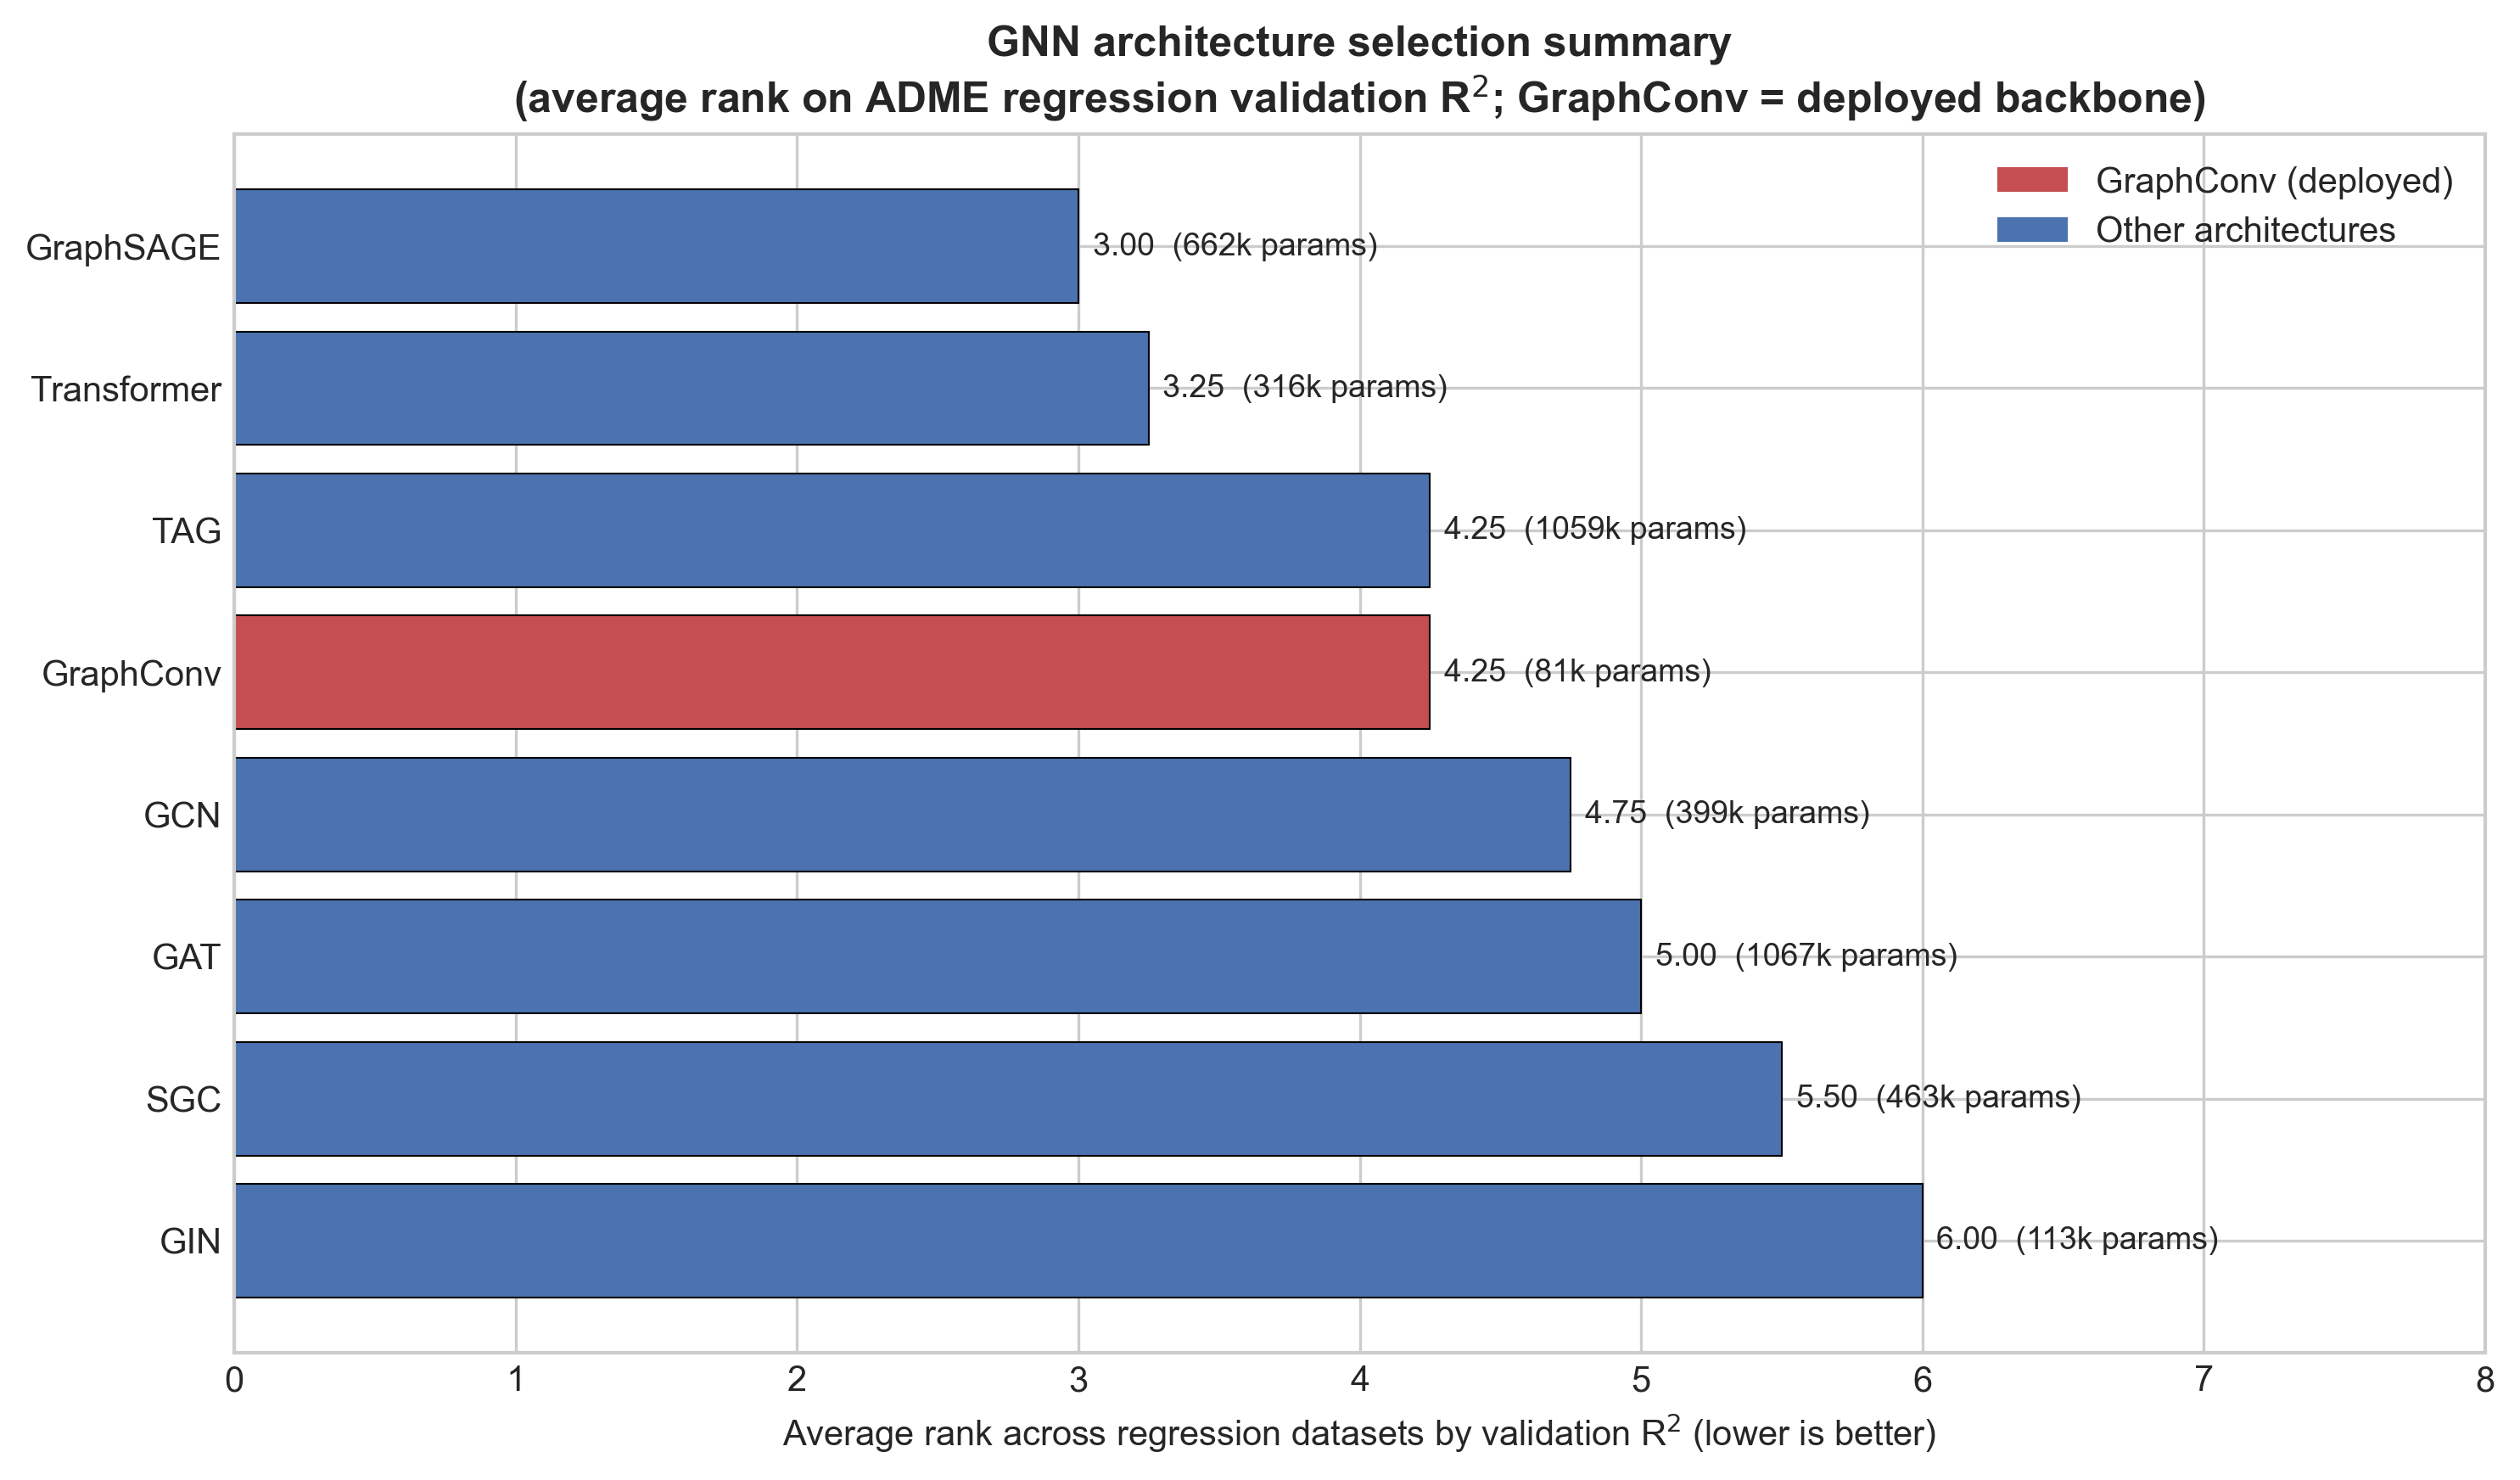
\includegraphics[width=0.95\textwidth,height=0.30\textheight,keepaspectratio]{arch_selection_summary.png}
    \caption{Preliminary architecture-selection summary showing average rank across the regression datasets by validation R$^2$ (lower is better); GraphConv (the deployed backbone) is highlighted. No architecture dominates and the per-dataset differences fall within the noise of these small datasets; GraphConv was adopted as a single representative backbone using validation metrics only.}
    \label{fig:arch_selection_summary}
\end{figure}

\begin{figure}[H]
    \centering
    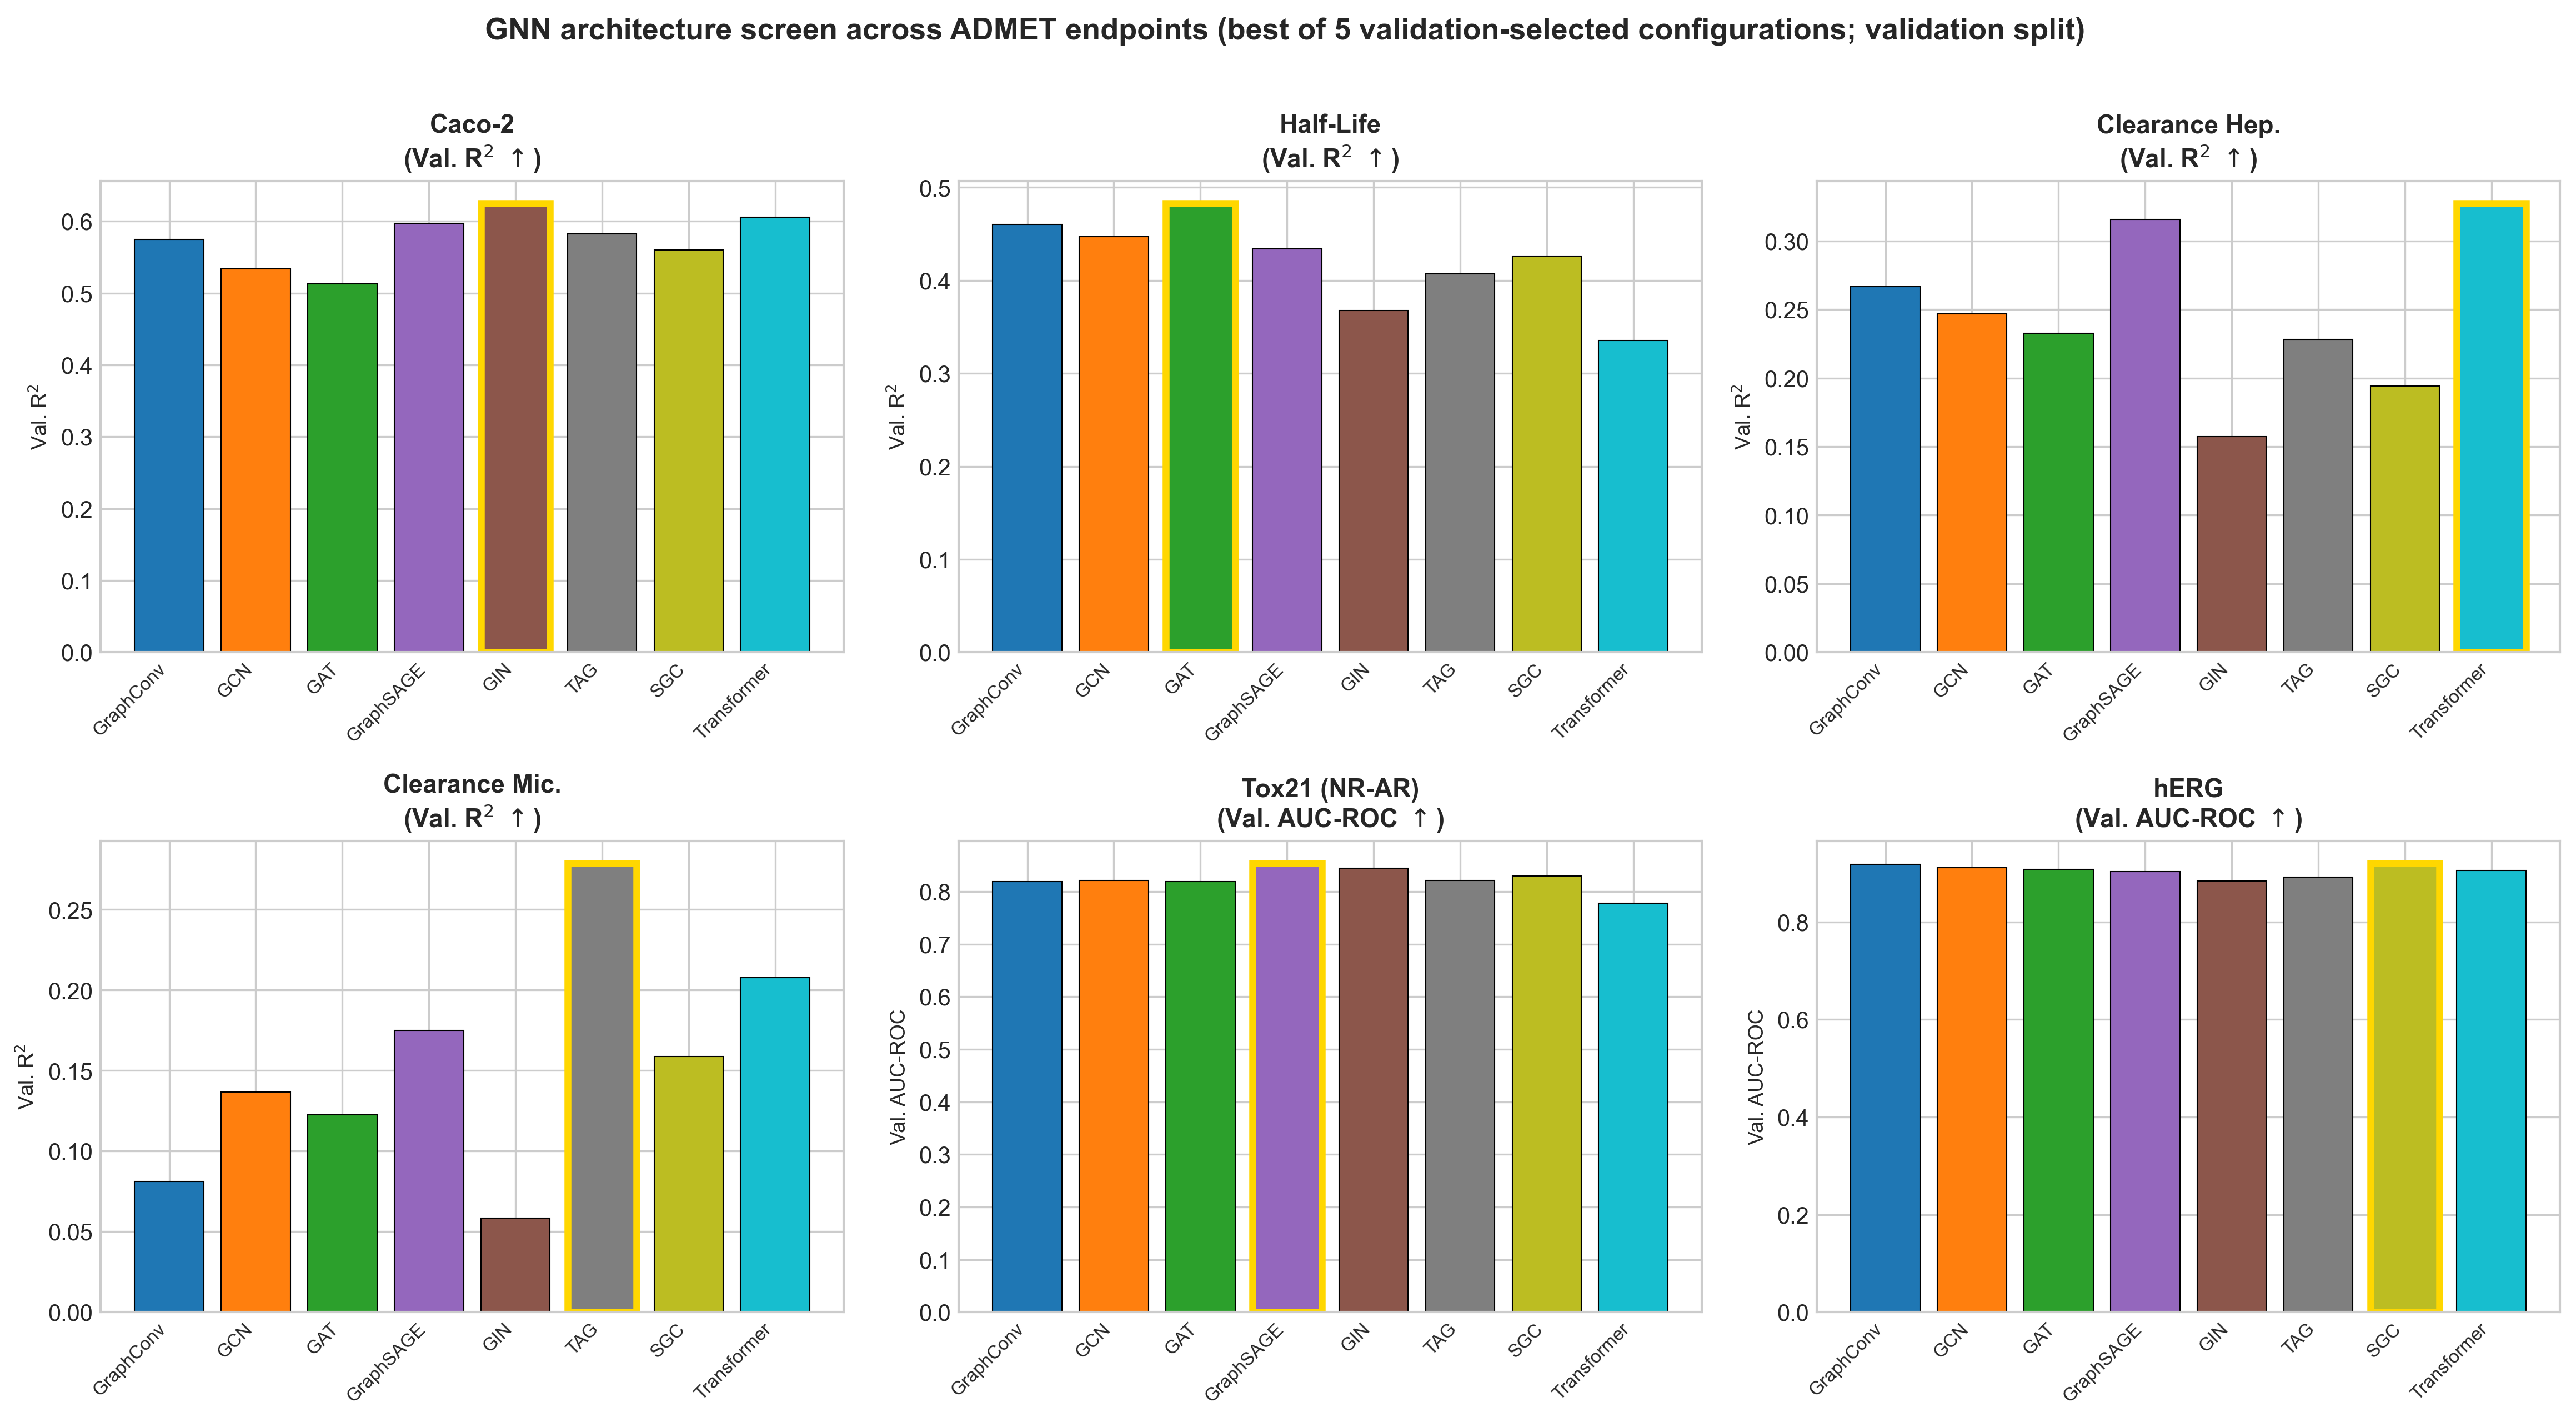
\includegraphics[width=0.95\textwidth,height=0.42\textheight,keepaspectratio]{arch_comparison_all_datasets.png}
    \caption{Per-dataset architecture comparison across all six benchmark endpoints. Classification endpoints (Tox21, hERG) are shown by validation AUC-ROC and regression endpoints (Caco-2, Half-Life, Hepatocyte and Microsomal Clearance) by validation R$^2$ (the selection basis). The weakly-learnable clearance and half-life endpoints are unstable across all eight architectures, whereas the structure-driven endpoints cluster within a narrow band.}
    \label{fig:arch_comparison}
\end{figure}

\end{document}
